\chapter{Bipolar Junction Transistor}

\section{Control Principle}

\begin{figure}[H]
  \centering
  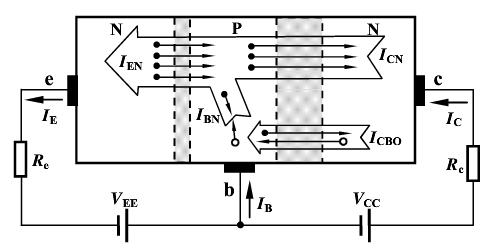
\includegraphics[width=0.5\linewidth]{figures/BJT-control-principle}
  \label{fig:}
\end{figure}

\begin{equation*}
  \begin{aligned}
    \alpha &= \dfrac{I_{CN}}{I_E} \\
    \beta &= \dfrac{I_{CN}}{I_{CBO}} 
  \end{aligned}
\end{equation*}

\section{Three Types of Amplifier Circuit}

\begin{figure}[H]
  \centering
  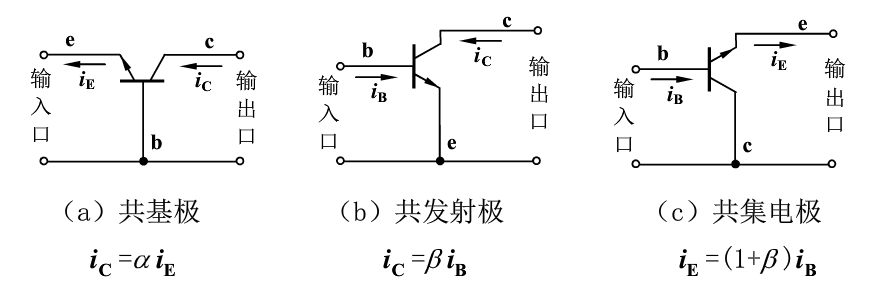
\includegraphics[width=0.9\linewidth]{figures/BJT-three-types}
  \label{fig:}
\end{figure}

\section{Static Working Point}

\begin{figure}[H]
  \centering
  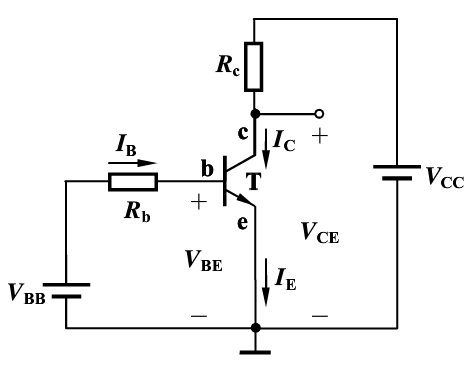
\includegraphics[width=0.4\linewidth]{figures/BJT-static}
  \label{fig:}
\end{figure}

\begin{equation*}
  \begin{aligned}
    & I_{BQ} = \dfrac{V_{BB} - V_{BEQ}}{R_b} \\
    & V_{BEQ} = 0.7 \  \mathrm{V} \\
    & I_{CQ} = \beta I_{BQ} \\
    & V_{CEQ} = V_{CC} - I_{CQ} R_{C}
  \end{aligned}
\end{equation*}

Note that the static working point is not associated with small signals discussed below.

\section{Model of Small Signal}

\begin{figure}[H]
  \centering
  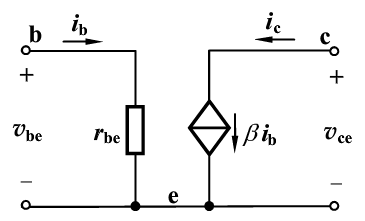
\includegraphics[width=0.4\linewidth]{figures/BJT-small-signal}
  \label{fig:}
\end{figure}

When $T = 300 \  \mathrm{K}$

\begin{equation*}
  \begin{aligned}
    r_{be} = 200 \  \Omega + \left( 1 + \beta \right) \dfrac{26 \  \mathrm{mV}}{I_{CQ} \left( \mathrm{mA} \right)} 
  \end{aligned}
\end{equation*}

\section{Compound Transistor}

\begin{figure}[H]
  \centering
  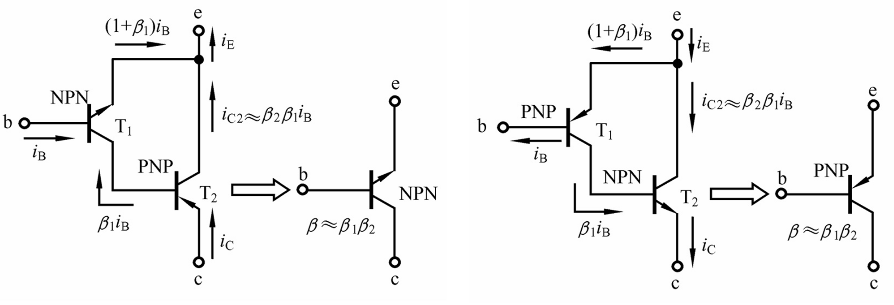
\includegraphics[width=0.7\linewidth]{figures/BJT-compound}
  \label{fig:}
\end{figure}



%%% Local Variables:
%%% mode: latex
%%% TeX-master: "Analogue_Electronics"
%%% End:
